\documentclass[a4paper,12pt]{article}
 
\usepackage{cmap}		
\usepackage[utf8]{inputenc}			
\usepackage[english,russian]{babel}
\usepackage{framed}
\usepackage{hyperref}
\usepackage{amsmath}
\usepackage{graphicx}
\usepackage[colorinlistoftodos]{todonotes}
\usepackage{wrapfig}
\usepackage{lipsum}
\usepackage{color}
\usepackage{indentfirst}
\usepackage{times}
\usepackage{textcomp}
\usepackage{float}
\usepackage{listings}
\usepackage{xcolor}
\usepackage[T1]{fontenc}
 
\usepackage{morewrites}
 
\usepackage[pdf]{graphviz}
\usepackage{xpatch}
\makeatletter
\newcommand*{\addFileDependency}[1]{% argument=file name and extension
  \typeout{(#1)}
  \@addtofilelist{#1}
  \IfFileExists{#1}{}{\typeout{No file #1.}}
}
\makeatother
\xpretocmd{\digraph}{\addFileDependency{#2.dot}}{}{}
 
\usepackage[autosize]{dot2texi}
\usepackage{tikz}
\usetikzlibrary{shapes,arrows}

\title{Домашнее задание №3}
\author{Сабитов Сергей А-13а-19}

\begin{document}
\maketitle
\section{Машины Тьюринга}

Работу требуется выполнять в системе \url{turingmachine.io}. \\\\
Для сдачи заданий 1-2 требуется прикрепить файлы YAML с исходным кодом проекта. Каждый файлы должен иметь наименование задание\_пункт.yml, к примеру 1\_1.yml для первой задачи первого задания. \\\\

\subsection{Операции с числами}

Реализуйте машины Тьюринга, которые позволяют выполнять следующие операции:
\begin{enumerate}
    \item Сложение двух унарных чисел (1 балла)
    
   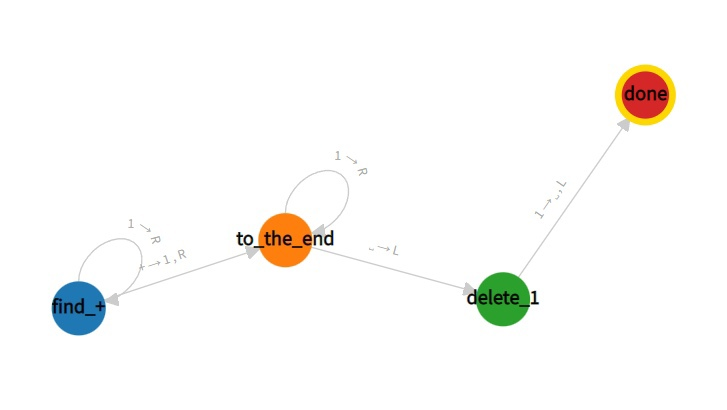
\includegraphics[scale=0.5]{11hw3.jpg}

    \item Умножение унарных чисел (1 балл)
    
    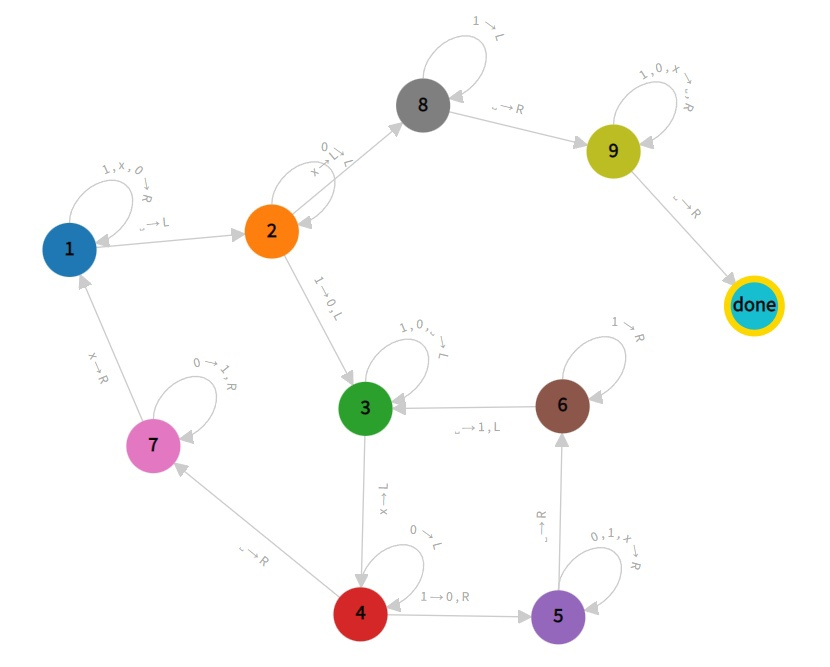
\includegraphics[scale=0.5]{12hw3.jpg}
\end{enumerate}


\subsection{Операции с языками и символами}

Реализуйте машины Тьюринга, которые позволяют выполнять следующие операции:
\begin{enumerate}
    \item Принадлежность к языку $L = \{ 0^n1^n2^n \}, n \ge 0$ (0.5 балла)
    
    МТ строится аналогично той, что мы строили на лекции
    
    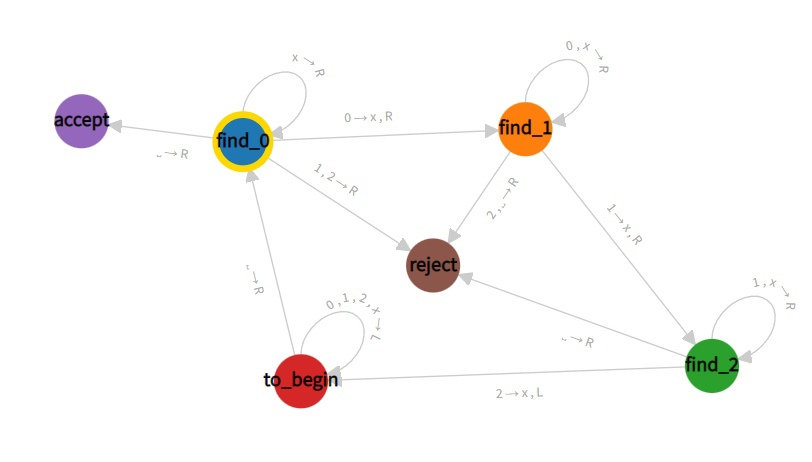
\includegraphics[scale=0.5]{21hw3.jpg}
    
    \item Проверка соблюдения правильности скобок в строке (минимум 3 вида скобок) (0.5 балла)
    
     МТ принимает последовательность скобок и в конце мы смотрим на конечное состояние: если это qA - то скобочная последовательность правильная; если qR - неправильная.
     
     Алгоритм заключается в том, что 
        \begin{itemize}
            \item мы считываем открывающую скобку и помечаем ячейку
            \item ищем соответствующую закрывающую и так же помечаем ячейку
            \item идем в начало до пустого символа и начинаем с 1 пункта
        \end{itemize}
    
    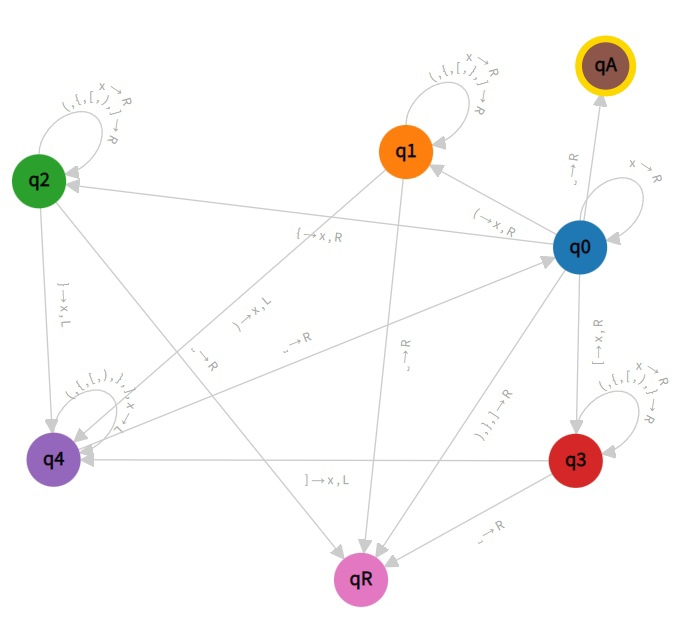
\includegraphics[scale=0.5]{22hw3.jpg}
    
    \item Поиск минимального по длине слова в строке (слова состоят из символов 1 и 0 и разделены пробелом) (1 балл)
\end{enumerate}


\section{Квантовые вычисления}


В качестве решения задачи надо предоставить схему алгоритма для частного случая при фиксированном количестве кубитов и фиксированных состояниях. 


\subsection{Генерация суперпозиций 1 (1 балл)}

Дано $N$ кубитов ($1 \le N \le 8$) в нулевом состоянии $\Ket{0\dots0}$. Также дана некоторая последовательность битов, которое задаёт ненулевое базисное состояние размера $N$. Задача получить суперпозицию нулевого состояния и заданного.

$$\Ket{S} = \frac{1}{\sqrt2}(\Ket{0\dots0} +\Ket{\psi})$$

То есть требуется реализовать операцию, которая принимает на вход:

\begin{enumerate}
    \item Массив кубитов $q_s$
    \item Массив битов $bits$ описывающих некоторое состояние $\Ket{\psi}$. Это массив имеет тот же самый размер, что и $qs$. Первый элемент этого массива равен $1$.
\end{enumerate}


Код:
\begin{lstlisting}
namespace Solution {
        open Microsoft.Quantum.Primitive;
        open Microsoft.Quantum.Canon;
        operation Solve (qs : Qubit[], bits : Bool[]) : ()
        {
            body
            {
                H(qs[0]);
                for (i in 1..Length(qs) - 1) {
                    if (bits[i]) {
                        CNOT(qs[0], qs[i]); 
                    } 
                } 
            }
        }
}
\end{lstlisting}

Схема для случая \(|0 0 0 0 \rangle\), \(|1 1 1 0 \rangle\): 
        \begin{center}
            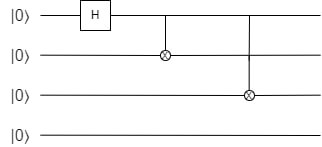
\includegraphics[scale=1]{31hw3.jpg}
        \end{center}
\subsection{Различение состояний 1 (1 балл)}

Дано $N$ кубитов ($1 \le N \le 8$), которые могут быть в одном из двух состояний:

$$\Ket{GHZ} = \frac{1}{\sqrt2}(\Ket{0\dots0} +\Ket{1\dots1})$$
$$\Ket{W} = \frac{1}{\sqrt N}(\Ket{10\dots00}+\Ket{01\dots00} + \dots +\Ket{00\dots01})$$

Требуется выполнить необходимые преобразования, чтобы точно различить эти два состояния. Возвращать $0$, если первое состояние и 1, если второе. 
\\\\
Код:
\begin{lstlisting}
namespace Solution {
        open Microsoft.Quantum.Primitive;
        open Microsoft.Quantum.Canon;
        operation Solve (qs : Qubit[]) : Int
        {
            body
            {
                mutable ones = 0;
                for (i in 0..Length(qs) - 1) {
                    if (M(qs[i]) == One) {
                        set ones = ones + 1;
                    }
                }
                if (ones == Length(qs) or ones == 0)
                {
                    return 0;
                }
                return 1;
            }
        }
}
\end{lstlisting}


\subsection{Различение состояний 2 (2 балла)}

Дано $2$ кубита, которые могут быть в одном из двух состояний:

$$\Ket{S_0} = \frac{1}{2}(\Ket{00} + \Ket{01} + \Ket{10} + \Ket{11})$$
$$\Ket{S_1} = \frac{1}{2}(\Ket{00} - \Ket{01} + \Ket{10} - \Ket{11})$$
$$\Ket{S_2} = \frac{1}{2}(\Ket{00} + \Ket{01} - \Ket{10} - \Ket{11})$$
$$\Ket{S_3} = \frac{1}{2}(\Ket{00} - \Ket{01} - \Ket{10} + \Ket{11})$$


Требуется выполнить необходимые преобразования, чтобы точно различить эти четыре состояния. Возвращать требуется индекс состояния (от $0$ до $3$). 
\\\\
Заготовка для кода:
\begin{lstlisting}
namespace Solution {
        open Microsoft.Quantum.Primitive;
        open Microsoft.Quantum.Canon;
        operation Solve (qs : Qubit[]) : Int
        {
            body
            {

                return 
            }
        }
}
\end{lstlisting}


\subsection{Написание оракула 1 (2 балла)}

Требуется реализовать квантовый оракул на $N$ кубитах ($1 \le N \le 8$), который реализует следующую функцию: $f(\pmb{x}) = (\pmb{b}\pmb{x}) \mod 2$, где  $\pmb{b} \in \{0,1\}^N$ вектор битов и  $\pmb{x}$ вектор кубитов. Выход функции записать в кубит $\pmb{y}$. Количество кубитов $N$ ($1 \le N \le 8$). 
\\\\
Заготовка для кода:
\begin{lstlisting}
namespace Solution {
        open Microsoft.Quantum.Primitive;
        open Microsoft.Quantum.Canon;
        operation Solve (x : Qubit[], y : Qubit, b : Int[]) : ()
        {
            body
            {

            }
        }
}
\end{lstlisting}
\end{document}